% %%%%%%%%%%%%%%%%%%%%%%%%%%%%%%%%%%%%%%%%%%%%%%%%%%%%%%
% In dieser Datei steht der Text fuer das gemeinsame 
% Einleitungs-Kapitel.
% %%%%%%%%%%%%%%%%%%%%%%%%%%%%%%%%%%%%%%%%%%%%%%%%%%%%%%

\section{Einleitung}%
\label{sec:einleitung}

Dies hier ist ein Blindtext zum Testen von Textausgaben.
Wer diesen Text liest, ist selbst schuld.
Der Text gibt lediglich den Grauwert der Schrift an.
Ist das wirklich so?
Ist es gleichgültig ob ich schreibe:
"Dies ist ein Blindtext" oder "Huardest gefburn"? Kjift mitnichten!
Ein Blindtext bietet mir wichtige Informationen. 
An ihm messe ich die Lesbarkeit einer Schrift, ihre Anmutung,
wie harmonisch die Figuren zueinander stehen und prüfe, wie breit oder schmal sie läuft. 
Ein Blindtext sollte möglichst viele verschiedene Buchstaben enthalten
und in der Originalsprache gesetzt sein. Er muss keinen Sinn ergeben, sollte
aber lesbar sein. Fremdsprachige Texte wie "Lorem ipsum" dienen nicht dem
eigentlichen Zweck, da sie eine falsche Anmutung vermitteln.


Abbildung~\ref{fig:mri} zeigt ein Beispiel für MR-Bilder.
Es gibt viel Literatur zur Normalisierung von Intensitäten in MR-Bildern (z.\,B.~\cite{Jaeger09}). 


\begin{figure}[h]
\centering
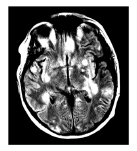
\includegraphics[height=4cm]{Grafiken/jaeger1.png}
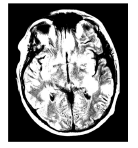
\includegraphics[height=4cm]{Grafiken/jaeger2.png}
\caption{Ein Beispiel für MR-Bilder (entnommen aus \cite{Jaeger09}).}%
\label{fig:mri}
\end{figure}
